\chapter{Introduzione}
\lstset{basicstyle=\small\ttfamily,keywordstyle=\color{black}\bfseries,commentstyle=\color{darkgray},stringstyle=\color{black},showstringspaces=true}

Con questa tesi si ha come obbiettivo di studiare e analizzare le varie tecniche di spam detection ed in particolare analizzare le tecniche online. Le tecninche verrano classificate sulla base dei segnali che utilizzano. Il fattore chiave è che non ci sono, o meglio sono poche, al momento tecniche online di spam detection, ovvero tecninche che rilevano lo spam durante la fase di crawling. Infatti quasi tutti i metodi tentano di fare il crawling dell'intero web e successivamente classificare le pagine in spam oppure buone.

Il feonomeno del web spam è sempre più presente all'interno del web. Questo è dovuto al fatto che gli utenti tendono ad esaminare solo i primi risultati ritornati dai motori di ricerca e quindi se un sito fa parte dei primi risultati di una un motore di ricerca ha un ritorno economico legato alla quantità di traffico che viene generata per quel sito. Uno studio  del 2005 descritto in \cite{Nicholas:2005}, stima che la perdita finanziaria mondiale causata dallo spam e di circa 50 miliardi di dollari e nel 2009 (come descritto in \cite{Nicholas:2009}) è salita a 130 miliardi di dollari.

Recentemente tutte le più grandi compagnie di motori di ricerca hanno identificato il recupero di informazioni non pertinenti come una delle priorità da risolvere. Le conseguenze del web spam possono essere \cite{Spirin:2012:SWS:2207243.2207252}:
\begin{itemize}
 \item la qualità delle ricerche è compromessa penalizzando i legittimi siti web;
 \item un utente podrebbe perdere la fiducia sulla qualità di un motore di ricerca e perciò passare con facilità all'utilizzo di un altro;
 \item inoltre i siti spam possono essere usati come mezzo per malware, pubblicazione di contentuto per adulti e attacchi di tipo ``fishing''.Un prova tangibile si può vedere in \cite{Eiron:2004:RWF:988672.988714}, dove gli autori hanno eseguito l'algoritmo di PageRank su 100 milioni di pagine e hanno notato che 11 su i primi 20 risultati erano composti da siti pornogragici.
\end{itemize}
Queste considerazioni evidenziano che quando si progetta un motore di ricerca bisogna tenere conto delle pagine che potrebbero portare al mal funzionamento del motore stesso.

Il lavoro prodotto sarà utilizzato per essere integrato	all'interno di un web crawler distribuito ad alte prestazioni. L'esigenza di tale modulo è sorta a seguito dello sviluppo, presso il Dipartimento, di un crawler chiamato {\itshape BubiNG}, altamente configurabile ma privo al momento di qualunque forma di rilevazione di siti e contenuti malevoli. Il problema è estremamente interessante sia dal punto di vista teorico che da quello pratico: infatti, sebbene
siano numerose le tecniche descritte in letteratura per la determinazione di spam (usando come segnali sia il contenuto che la struttura dei link), è sorprendentemente scarso l'insieme di tali tecniche che possono essere usate on-line durante il crawl. Il problema diventa ancora più complesso se si aggiungono considerazioni legate ai vincoli di spazio di memoria disponibile e tempo di calcolo.
Infatti in lettaratura il processo di spam detection viene eseguito subito dopo la fase di crawling. Ovvero il processo è composto dai seguenti passi:
\begin{itemize}
 \item crawling dell'intero web;
 \item fase di spam detection;
 \item indicizzazione.
\end{itemize}
Questo modello è utile perché molte delle tecniche utilizzate fanno delle analisi sul grafo che risulta alla fine del processo di crawling. Da queste considerazioni noi proviamo a fare delle analisi per determinare se il processo di spam detection può essere fatto durante la fase di crawling ovvero al momento in cui il crawler esegue il ``fetch'' di una pagina determinare ``on the fly'' se la pagina è buona o ha un contenuto malevolo. 

\section{Ranking dei motori di ricerca}
Prima di spiegare i vari metodi per fare web spam e successivamente quelli utili ad identificarlo, è necessario capire come i motori di ricerca sono capaci di valutare la rilevanza di una pagina web per una determinta query.
%preso dalle dispense

In linea di massima un sistema di reperimento di informazioni ovvero un motore di ricerca è dato da una collezione documentale \textit{D} (un insieme di documenti) di dimensione \textit{N} , da un insieme \textit{Q} di interrogazioni, e da funzione di ranking (\(r : Q \times D \mapsto R\)) che
assegna a ogni coppia formata da un’interrogazione e un documento un numero reale. L’idea è che a fronte di un’interrogazione a ogni documento viene assegnato un punteggio reale: i documenti con punteggio nullo non sono considerati rilevanti, mentre quelli a punteggio non nullo sono tanto più rilevanti quanto il punteggio è alto. In particolare i metodi di ranking si dividono in \textit{endogeni} ed \textit{esogeni}. I primi metodi fanno uso del contenuto del documento per valutarne la rilevanza mentre i secondi fanno uso di un struttura esterna che nel caso del web si rififerisce al grafo composto dai collegamenti ipertestuali tra le pagine. Tra i metodi esogeni sono di maggiore importanza \textit{tf-idf} e \textit{BM25} mentre tra quelli esogeni i più diffusi in letteratura sono \textit{PageRank} e \textit{HITS}.

\subsection{Metodi di ranking endogeno}
L'algoritmo usato dai motori di ricerca per fare il rank delle pagine web basandosi sui campi di testo usa varie forme del \textit{tf-idf}. Il \textit{tf-idf} e un metodo di ranking endogeno che utilizza il contenuto di una pagina per assegnarle un punteggio. Il \textit{tf-idf} è una misura composta da due misure più semplici: la \textit{Term Frequency} e la \textit{Inverse Document Frequency}. Il primo metodo assegna a un documento \textit{d} il punteggio dato dalla somma dei conteggi dei termini \textit{t} dell'interrogazione che compaiono nel documento stesso. In questo modo documenti che hanno termini che compaiono più frequentemente avranno un punteggio più elevato. Utilizzare solo questo metodo non conviene in quanto è facilmente manipolabile. Inoltre non tiene cono del fatto che alcuni termini occorono più frequentemente non perché rilevanti, ma perché altamente frequenti all'iterno di \textit{ogni} documento. Ad esempio le congiunzioni. Il secondo metodo è definito come l'inverso del numero di 
documenti nella collezione che contengono il termine \textit{t} \cite{Manning:2008:IIR:1394399p117}.
\begin{equation}
 idf_t=\log\frac{N}{df_t}
 \label{eq:idf}
\end{equation}
La combinazione del \textit{TF} ed dell' \textit{IDF} produce una misura composta che permette di normalizzare il peso dei termini. Il \textit{TF-IDF} di un documento \textit{d} rispetto a uan query \textit{q} è calcolato su tutti i termini \textit{t} in comune come:
\begin{equation}
 tf-idf(d,q)=\sum_{t \in d \: and \: t \in q} tf(t) \cdot idf(t)
\end{equation}
Con il \textit{TF-IDF} gli spammers possono avere due obbiettivi: o creare pagine rilevanti per un gran numero di query o creare pagine molto rilevanti per una specifica query. Il primo obbiettivo può essere finalizato includendo un gran numero di termini distinti in un documento. Il secondo attraverso la ripetizione di determinati nel documento. Ma il più delle volte i motori di ricerca non considerano l'\textit{IDF} e perciò per incrementare il \textit{TF-IDF} conviene incrementare la frequenza dei termini.

Anche se il \textit{tf-idf} riesce a pesare abbastanza bene i vari termini ha molti limiti e per questo che il sistema di pesatura più attualmente usato è \textit{BM25} che è uno schema di pesatura basato sul \textit{modello probabilistico}. Questo schema è il risultato di uno studio puramente euristico.

\subsection{Metodi di ranking esogeno}
Uno dei metodi esogeni è \textit{PageRank} descritto in \cite{ilprints422}. PageRank usa le informazioni portate dai link in entrata (\textit{inlink}) per determinare un punteggio gobale di importanza di una pagina. Esso assume che esiste un legame tra numero di \textit{inlink} di una pagina \textit{p} e la popolarità della pagina \textit{p}. Il concetto fondamentale dietro \textit{PageRank} è che una pagina è importante se moltre altre pagine importanti puntano ad essa. Questo concetto è mutualmente rinforzante ovvero l'importanza di una certa pagina influenza ed è influenzata dall'importanza delle altre pagine \cite{ilprints646}. In dettaglio \textit{PageRank} è basato sulla passeggiata naturale del grafo del web \textit{G}. Più precisamente, la passeggiata viene pertubata nel seguente modo: fissato un parametro \(\alpha\) tra \(0\) e \(1\), a ogni passo con probabilità \(\alpha\) si segue un arco uscente, e con probabilità \(1- \alpha \) si sceglie un qualunque altro nodo del grafo utilizzando una qualche 
distribuzione \(v\), detta
vettore di preferenza (per esempio, uniforme). Assumendo che non esistano pozzi, la catena è quindi rappresentata dalla combinazione lineare:
\begin{equation}
 \alpha G + (1 - \alpha) 1 v^T
\end{equation}
dove \(G\) è la matrice della passeggiata naturale su \(G\). Il fattore \(\alpha\) è detto fattore di attenuazione di norma è impostato a unvalore di 0,85.

Un altro metodo usato per il ranking delle pagine è \textit{HITS (Hyperlink-Induced Topic Distillation)} introdotto in \cite{Kleinberg:1999:ASH:324133.324140}. Differentemente da \textit{PageRank} esso assegna due punteggi di scrore a ogni pagina: uno di \textit{hubbines} e uno di \textit{autorevolezza}. L’intuizione dietro a HITS è che invece di un singolo punteggio di autorevolezza esista un concetto di pagina autorevole, cioè pagina con contenuto pertinente e interessante, e di hub, cioè pagina contenente numerosi collegamenti a pagine autorevoli. I due concetti si rinforzano \textit{mutuamente}: una pagina autorevole è puntata da molte pagine centrali, e una buona pagina centrale punta a molte pagine autorevoli.

Questo approccio considera che nel web ci sono due tipi di pagine: quelle che contengono dei contenuti per un determinato argomento (\textit{authoritative}) e quelle che contengono tanti link a delle pagine \textit{authoritative} che sono chiamate pagine \textit{hub}. Le pagine \textit{hub} sono utili per scoprire le pagine \textit{authoritative} \cite{Manning:2008:IIR:1394399p474}.

L'algoritmo parte da un sottografo del web ottenuto a partire da un'interrogazione. La selezione del sottografo può essere fatta in vari modi, un modo è quello di prendere un certo insieme di risultati  ottenuto da un motore di base e generare un sottografo sulla base di una query e delle pagine che puntano a quelle ottentute dalla query. Per questo sottoinsieme di pagine otteniamo un matrice di adicenza \(A\). I punteggi di \textit{hub} e \textit{authority} per tutte le pagine del sottoinsieme possono essere formalizzate dalla seguente coppia di equazioni:
\begin{equation}
 \left\{
 \begin{array}{cc}
    \stackrel{\rightarrow}{a} \: = \: A^T \stackrel{\rightarrow}{h}\\
    \stackrel{\rightarrow}{h} \:= A \: \stackrel{\rightarrow}{a}
 \end{array}
 \right .
 \label{eq:hubat}
\end{equation}
Può essere dimostrato che la soluzione per il sistema di equazioni \ref{eq:hubat} dopo una serie iterativa di calcoli converge rispettivamente al principale autovettore di \(AA^T\) e \(A^TA\) \cite{Manning:2008:IIR:1394399p474}\cite{Spirin:2012:SWS:2207243.2207252}.

\section{Web spam}
Con il termine web spamming si fa riferimento a tutti i metodi che tentano di manipolare gli algoritmi di ranking dei motori di ricerca per aumentare il valore di ranking di alcune pagine rispetto ad altre\cite{ilprints646}.
Dato il numero esorbitante di pagine che vengono create e pubblicate sul web, gli utenti competono per poter far comparire le proprie pagine tra le prime dei risultati di una query.
Il fenomedo dello spamming o spamindexing comporta che la qualità delle ricerche decrementa, gli utenti tenderanno ad utilizzare altri motori di ricerca, l'indicizzazione di pagine che non sono utili e l'aumento del costo delle operazioni di query ed infine la causa di malware e reindirizzamento verso contenuto per adulti\cite{Spirin:2012:SWS:2207243.2207252}.

L'obbiettivo del motori di ricerca è di ottenere ottimi risultati per identificare tutte le pagine web che sono rilevanti per una specifica query e presentarle secondo l'importanza che esse hanno. Di norma la rilevanza viene misurata attraverso la similarità testuale tra la query e le pagine mentre l'importanza è definita come la popolarità globale della pagina e a volte è inferita dalla struttura dei link \cite{ilprints646}. Ci sono due categorie di tecniche associate al web spam \cite{ilprints646}:
\begin{itemize}
\item \textbf{tecniche boost} che cercano di far avere più importanza o rilevanza a delle pagine
\item \textbf{tecniche hiding} che sono metodi per nascondere le tencinche di boost all'utente dal browser, anche se alcuni autori incorporano queste tecniche facenti parte delle tecniche di boost
\end{itemize}

\subsection{Tecniche di boost}
Le tecninche di boosting si dividono in: \textit{Term Spamming} e \textit{Link Spamming}. Con l'avvento degli algoritmi di ranking basati sulla struttura del grafo il textit{Term Spaming} è stato trascurato. In figura \ref{fig:tassonomiaTecnicheBoost} è specificata la tassonomia delle tecniche boost \cite{ilprints646}.
\begin{figure} 
 \centering
 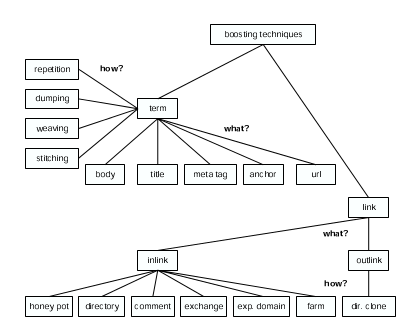
\includegraphics[width=10cm]{immagini/tassonomiaTecnicheBoost}
 \caption{Tassonomia delle tecniche boost}
 \label{fig:tassonomiaTecnicheBoost}
\end{figure}

\subsection{Term Spamming}
Nel valutare la rilevanza testuale i motori di ricerca considerano dove i termini di una query compaiono in una pagina. Il tipo di punto all'interno della pagina è chiamato \textit{campo}. I più comuni campi di testo per una pagina \textit{p} sono: il body della pagina, il titolo, i meta tag nell'header HTML e l'URL della pagina. Inoltre il testo delle ancore (il tag \textit{a}) associate all'URL che puntano alla pagina \textit{p} sono considerati dal momento che possono descrivere molto bene il contenuto della pagina. I campi di testo  di \textit{p} sono utilizzati per detrminare la rilevanza di \textit{p} rispetto ad una query alcune volte con differenti proporziona. Il term spamming utilizza tecniche di pesatura dei contenuti dei campi di testo in modo tale da creare pagine di spam rilevanti per delle query \cite{ilprints646}.

Le tecninche di spamming possono essere raggruppate in base ai campi di testo dove viene fatto spamming. In base a questo distinguiamo:
\begin{itemize}
\item \textit{Body Spam}. In questo caso lo spam è nel corpo del documento. Questo è lo spam più diffuso.
\item \textit{Title Spam}. Molti motori di ricerca danno molta importanza ai termini che compaiono nel titolo.
\item \textit{Meta Tag Sapm}. I tag che compaiono nell'header sono soggetti a spam. Per questo i motori di ricerca danno poca importanza a questi campi o non li considerano. Di seguito viene mostrato un esempio di spam.
\begin{lstlisting}[frame=trbl,postbreak=\space, breakindent=5pt, breaklines]
 <meta name=``keyword'' content=``buy, cheap, cameras, lens, accessories, nikon, canon''>
\end{lstlisting}
\item \textit{Anchor Text Spam}. I motori di ricerca assegnano un peso maggiore al testo nelle ancore perché pensano esse contengano un riassunto del contenuto della pagina. Perciò testo di spam è incluso nel testo delle ancore dei collegamenti HTML di una pagina. In questo caso lo spamming non viene fatto sulla pagina che si vuole far avere un rank più alto ma sulle pagine che puntano ad essa.
\begin{lstlisting}[frame=trbl,postbreak=\space, breakindent=5pt, breaklines]
<a href=``target.html">free, great deals, cheap, inexpensive, cheap, free</a>
\end{lstlisting}
\item \textit{URL Spam}. Alcuni motori di ricerca dividono l'URL delle pagine in un insieme di termini che sono usati per determinare la rilevanza di una pagina. Per sfruttare questo si creano lunghi URL che includono una grande sequenza di spam di termini un esempio può essere: \textit{buy-canon-rebel-20d-lens-case.camerasx.com}.
\end{itemize}
Queste tecniche possono essere utilizzate insieme.

Un altro modo per raggruppare queste tecniche si basa su che tipo di termini vengono utilizzati nei campi di testo. In questo modo vengono raggrupate in:
\begin{itemize}
\item \textit{Ripetizione di uno o più specifici termini.}
\item \textit{Inclusione di molti termini generici per creare pagine rilevanti per molte query.}
\item \textit{Intreccio di vari termini all'interno della pagina.}
\item \textit{Creazione di frasi per creare contenuti veloci attraverso la concatenazione di frasi da fonti diverse.}
\end{itemize}

\subsection{Link Spamming}
In \cite{ilprints646} viene definito che per uno spammer ci sono tre tipi di pagine nel Web: inaccessibili, accessibili(blog), proprietarie. Le inaccessibili sono quelle che uno spammer non può modificare. Le accessibili sono pagine gestite da altri ma che possono essere modificate un po' dallo spammer. Le proprietarie sono pagine degli spammer che hanno il pieno controllo. Il gruppo di pagine proprietarie è chiamato \textit{spam farm} \begin{math} \Sigma \end{math}.

Di norma i motori di ricerca utilizzano due algoritmi di ricerca per aumentare l'importanza basandosi sulle informazioni dei link: PageRank e HITS. %spiegazione

Ci sono due categorie principali di link spam: outgoing link spam e incomign link spam.

\textbf{Outgoing link}. E' uno dei metodi più facili da implementare in quanto basta aggiungere dei link a pagine conosciute considerate buone, sperando di poter aumentare il loro hub score. Per fare questo si possono utilizzare delle directory che contengono liste di siti come DMOZ o Yahoo!. Queste directory organizzano i contenuti web in contenuti e in liste di siti relativi.

\textbf{Incoming link}. Ci sono diverse strategie che si possono adottare in modo tale da avere un numero elevato di link in entrata:
\begin{itemize}
\item \textit{Honeypot}: ovvero si creano un insieme di pagine che hanno un contenuto interessante (un esempio può essere una documentazione Linux) ma che hanno link nascosti alla pagina o alle pagine per cui  deve aumentare il valore di rilevanza.  
\item \textit{Infiltrarsi in una directory web}: molte directory web permettono ai webmasters di postare links ai loro siti che honno lo stesso contenuto.
\item \textit{Postare link nei blog, forum e wiki}: includere URL a pagine di spam come parte di un commento.
\item \textit{Scambio di link}: scambiare link con altre pagine di spam.
\item \textit{Comprare domini scaduti}: quando un dominio scade ci sono delle pagine che puntano ancora ad esso. Comprando questi domini e riempirli di spam ha dei vantaggi per la rilevanza che si acquisice dai link che puntano ancora ad essa	.
\item Creare una spam farm: con l'abbassamento dei costi si possono costruire delle spam farm che hanno come obbietivo di aumentare la rilevanza delle pagine di spam. Molte volte si utilizzano tecninche come il vaso di miele. In questo caso il valore di page rank aggregato delle pagine è propagato alla pagina che hanno come link. Delle forme più aggressive di honeypot è l'hijacking\cite{Spirin:2012:SWS:2207243.2207252}. dove gli spammers prima attaccano un sito con una buona reputabilità e poi usano questo come parte della loro link farm.
\end{itemize}

\subsection{Click Spamming}
Dal momento che i motori di ricerca utilizzano i dati sul flusso di click per regolare le funzioni di ranking, gli spammers generano clik fraudolenti per manipolare il comportamento di queste funzioni in modo tale da fare avere un migliore rank i loro siti. Vengono fatte delle query e si clicca sulla pagina che si vuole aumentare il rank. Questo viene fatto in modo automatico attraverso script che girano su diverse macchine per non fare sospettare di tale comportamento.

\subsection{Tecninche di hiding}
Le tecninche di hiding si possono classificare in: content hiding, cloaking, redirection.

Content hiding. I termini o link di spam possono essere nascosti quando il browser visualizza una pagina. Una tecnica è quella di utilizzare lo stesso colore per i termini e lo sfondo. Mentre per i link basta non inserire il testo all'interno delle ancore che indirizzano a una pagina. Un'altra tecninca è quella di utilizzare degli script per nascondere il contenuto.

Cloaking. E' facile identificare quando la richiesta di una pagina è fatta da un crawler o da un browser per questo si utilizza questa tecninca che dato un URL il server spam restituisce un diverso documento HTML a seconda se la richiesta è fatta da un crowler o un browser. Cosi all'utente viene presentata una pagina con del contenuto mentre si manda un documento di spam al motore di ricerca. La rilevazione di crowler può essere fatta in due modi: o si mantiene in memoria una lista di indirizzi di crawler oppure attraverso l'header della richiesta HTTP andando a vedere il campo user-agent se questo è diverso dai pi comuni browser allora può essere un crawler.

Redirection. Un altro modo è quello di reindirizzare il browser ad un altro URL appena la pagina è caricata.

